\documentclass[main.tex]{subfiles}

\begin{document}

\section{Aufgabe 2}
Entscheiden Sie, ob die folgende Funktion auf dem Intervall $[-1;1]$ gleichmäßig stetig ist

\begin{equation*}
    f(x) =\frac{x}{4-x^{2}}
\end{equation*}

\subsection{Lösung 2}

\textcolor[rgb]{0.4,0.72,0.06}{Die Funktion$\displaystyle f( x)$ ist an der Stelle $\displaystyle x_{0}$ stetig, falls\begin{equation*}
    \forall \epsilon  >0\exists \delta ( x_{0} ,\epsilon )  >0\ :\ \forall ( x-x_{0}) < \delta \ :\ | f( x) -f( x_{0})| < \epsilon \text{.}
\end{equation*}
}

Die Funktion $f(x)$ ist \textbf{gleichmäßig stetig} in einem Intervall $D$, wenn in jedem Punkt $x_{0} \in D$ gilt:
\begin{equation*}
    \forall \epsilon  >0\exists \delta ( \epsilon )  >0\forall x,x_{0} \in D:(| x-x_{0}| < \delta ( \epsilon ) \Longrightarrow | f( x) -f( x_{0})| < \epsilon )\text{.}
\end{equation*}

Hinweis: Dabei muss $\delta $ unabhängig von $x_{0}$ sein.\\

\begin{figure}[ht]
	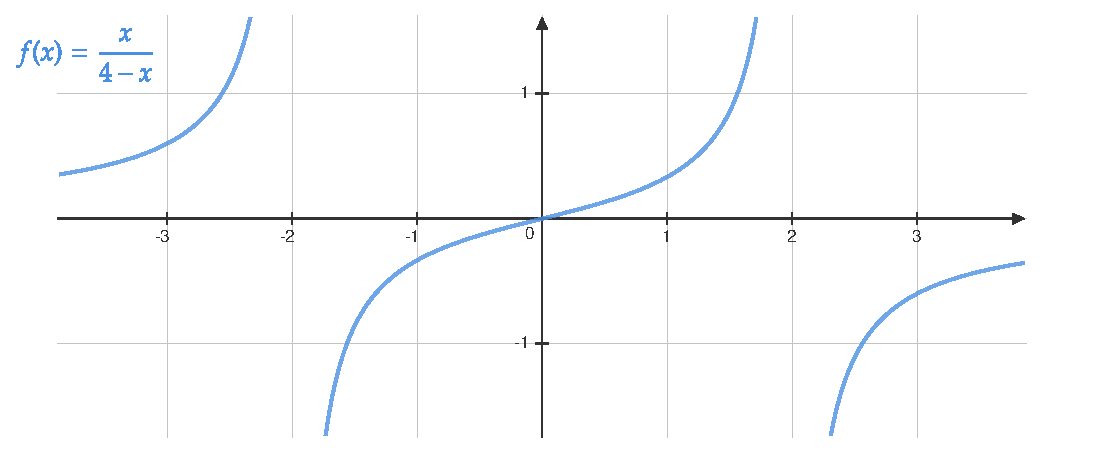
\includegraphics[width=\linewidth]{fig-2.pdf}
	\caption{Graph von $f(x)$}
\end{figure}

Stetigkeit mit $\epsilon $-$\delta $-Beweis zu zeigen. Sei $\epsilon >0$ und $x_{0} \in [-1;1]$
\begin{equation*}
	\begin{array}{ c r c l }
		& \ | f( x) -f( x_{0})|  & \equiv  & \left| \frac{x}{4-x^{2}} -\frac{x_{0}}{4-x_{0}^{2}}\right| \\
		&  & = & \left| \frac{x\cdotp \left( 4-x_{0}^{2}\right) -x_{0} \cdotp \left( 4-x^{2}\right)}{\left( 4-x^{2}\right) \cdotp \left( 4-x_{0}^{2}\right)}\right| \\
		&  & = & \left| \frac{4x-x_{0}^{2} x-4x_{0} +x_{0} x^{2}}{\left( 4-x^{2}\right) \cdotp \left( 4-x_{0}^{2}\right)}\right| \\
		&  & = & \left| \frac{( 4x-4x_{0}) +x_{0} x^{2} -x_{0}^{2} x}{\left( 4-x^{2}\right) \cdotp \left( 4-x_{0}^{2}\right)}\right| \\
		&  & = & \left| \frac{4( x-x_{0}) +( x-x_{0}) x_{0} x}{\left( 4-x^{2}\right) \cdotp \left( 4-x_{0}^{2}\right)}\right| \\
		&  & = & \left| \frac{( x-x_{0}) \cdotp ( 4+x_{0} x)}{\left( 4-x^{2}\right) \cdotp \left( 4-x_{0}^{2}\right)}\right| \\
		&  & = & \frac{\overbrace{| x-x_{0}| }^{\delta } \cdotp \overbrace{| 4+x_{0} x| }^{\leq \ 5}}{\underbrace{\left| 4-x^{2}\right| }_{\geq 3} \cdotp \underbrace{\left| 4-x_{0}^{2}\right| }_{\geq 3}}\\
		&  & \overset{x,x_{0} \in [ -1;1]}{\leq } & \frac{\delta \cdotp 5}{3\cdotp 3}\\
		&  & = & \frac{5}{9} \cdotp \delta \\
		&  & <  & \epsilon \\
		\Leftrightarrow  & \delta  & <  & \frac{9}{5} \cdotp \epsilon 
	\end{array}
\end{equation*}

Unter Verwendung des Intervalls konnte $\delta (\epsilon)$ abgeschätzt und allein in Abhängigkeit von $\epsilon $ angegeben werden. Somit ist die Funktion im Intervall gleichmäßig stetig.

\end{document}
